\documentclass{article}
\usepackage{graphicx} %package to manage images
\usepackage[utf8]{inputenc}
\usepackage[a4paper, total={6in, 8in}]{geometry}
\usepackage{xurl}
\usepackage{float}
\title{Relatório 13 \\ Ajuste Gaze.Event.duration}
\author{Pedro A. S. O. Neto}
\date{Outubro, 2022}

\begin{document}

\maketitle

\section{Tempo total de fixação (Gaze.Event.duration) - Inconsistências}

Foram identificadas inconsistências entre o tempo de fixação e o tempo de duração total de cada vídeo. Em alguns casos, o tempo total de fixção é maior do que a duração do vídeo.

\section{Identificação do problema}

Eu, Victor e Katerina investigamos a causa da inconsistência, e identificamos que as fixações não estavam divididas por vídeo, e sim por timeline. Isto é, em alguns casos, é possível que a fixação se inicie no video 1, e se extenda até o vídeo 2.

\section{Solução}

Já que o dado "Gaze.Event.duration" tem um spill-over entre trials, nossa solução foi computar o tempo de duração de cada fixação de acordo com o Computer.timestamp. O cálculo de duração de cada fixação é feito como a diferença entre o último e o primeiro time-stamp da fixação. Por fim, adicionamos 83ms a cada uma das fixações, que é o tempo entre cada sample feito pelo Tobii.

\section{Resultados}

Ainda assim, existem alguns (poucos) casos onde a duração das fixações é maior (pouco maior) do que a duração dos vídeos (Figura 1).

\begin{figure}[]
  \caption{Proporcão de fixações versus tempo do vídeo. Valores maiores do que 1, indicam um tempo de fixação maior do que a duração do próprio vídeo.}
  \noindent\makebox[\textwidth]{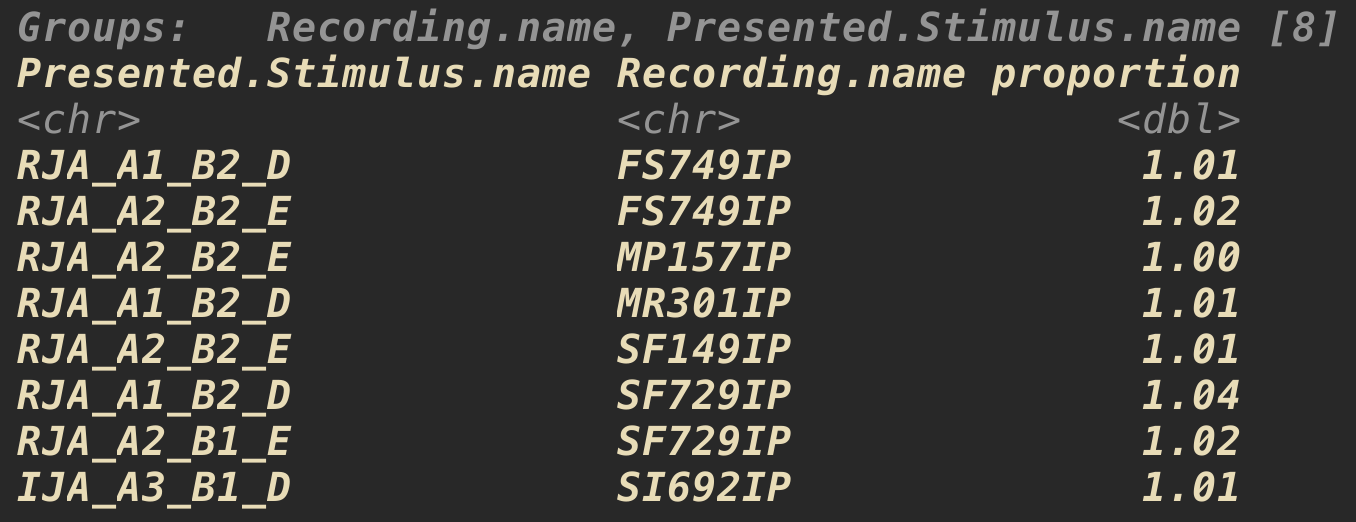
\includegraphics[scale=0.6]{./remainingProblems.png}}
  \centering
\end{figure}

Para verificar se a diferença entre o tempo de duração do vídeo e o tempo de fixação não se origina de algum problema nos códigos, ou algum problema de lógica das nossas análises, nós computamos outra medida indicativa da duração de cada vídeo.

\begin{figure}[]
  \caption{Marcação do Tobii para início e fim de cada vídeo.}
  \noindent\makebox[\textwidth]{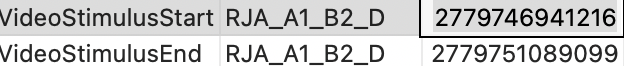
\includegraphics[scale=1]{./rawData.png}}
  \centering
\end{figure}

\begin{figure}[]
  \caption{Exemplo do cálculo de duração para cada vídeo. Neste caso, o vídeo tem uma duração de 4.14 segundos, sendo que a duração do vídeo RJA_A1_B2_D, medida por nós, é de 4.05}
  \noindent\makebox[\textwidth]{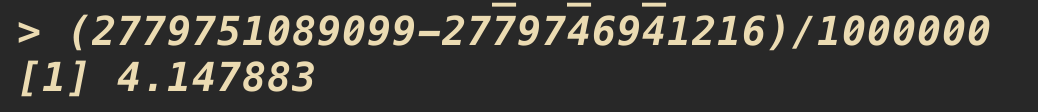
\includegraphics[scale=1]{./calculoDiferenca.png}}
  \centering
\end{figure}

As colunas "Event" e "Event.value" no raw data, indicam quando um vídeo começa e quando um vídeo termina. Nós medimos a duração de cada vídeo, para cada participante, e verificamos que, de fato, o problema está no raw data. 

\begin{figure}[]
\caption{Proporcão de fixações versus tempo do vídeo}
\noindent\makebox[\textwidth]{\includegraphics[scale=0.6]{./}}
\centering
\end{figure}

\section{Considerações finais}

As inconsistências encontradas no raw data são relativamente pequenas, e não devem influenciar muito ná análise macro. Porém, se pretendemos reportar "tempo de fixação" como uma variável de interesse, é importante que essas dúvidas sejam sanadas.

\end{document}
